\documentclass[tikz,border=5pt]{standalone}
\usepackage{amsmath}
\usetikzlibrary{arrows.meta,positioning,calc}

\begin{document}
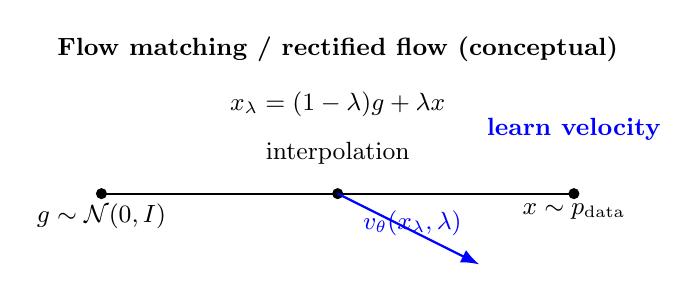
\begin{tikzpicture}[>=Latex, font=\small]
  \coordinate (g) at (0,0);
  \coordinate (x) at (6,0);
  \coordinate (m) at (3,0);

  % endpoints
  \fill (g) circle (2pt);
  \fill (x) circle (2pt);
  \node[below] at (g) {$g\sim\mathcal N(0,I)$};
  \node[below] at (x) {$x\sim p_{\mathrm{data}}$};

  % straight path
  \draw[thick] (g) -- (x);
  \node[above=0.25cm] at (m) {interpolation};

  % sample point on path
  \fill (m) circle (2pt);
  \node[above=0.85cm of m] {$x_\lambda=(1-\lambda)g+\lambda x$};

  % velocity arrow (conceptual)
  \draw[->, thick, blue] (m) -- ++(1.8,-0.9);
  \node[blue, below right=0.1cm and 0.2cm of m] {$v_\theta(x_\lambda,\lambda)$};
  \node[blue, above=0.55cm of x] {\textbf{learn velocity}};

  \node[above=1.55cm of m] {\textbf{Flow matching / rectified flow (conceptual)}};
\end{tikzpicture}
\end{document}


